%
% fig-ggz.tex -- eukldische Eigenschaft für ganze gaussche Zahlen
%
% (c) 2026 Prof Dr Andreas Müller
%
\begin{figure}
\centering
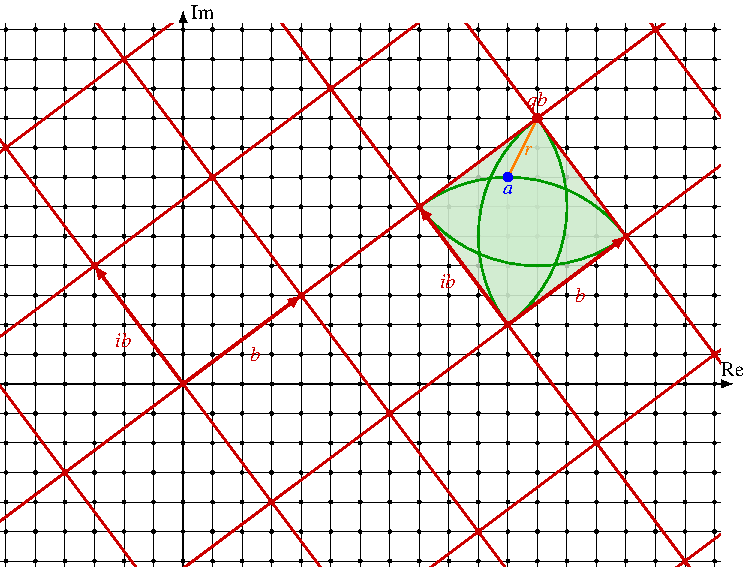
\includegraphics{chapters/060-ratint/images/ggz.pdf}
\caption{Euklidische Eigenschaft des Rings der ganzen gaussschen Zahlen.
Die Vielfachen $\mathbb{Z}[i]b= \{xb+y ib\mid x,y\in\mathbb{Z}\}$
bilden ein quadratisches Gitter ({\color{darkred}rot}). 
Die Zahl $a$ ({\color{blue}blau}) muss in einem der Gitterquadrate
({\color{darkgreen}grün}) liegen, die Seitenkanten $b$ und $ib$ haben.
Da die Kreise mit Radius $|b|$ um die Ecken das ganze Quadrat überdecken,
gibt es eine Ecke, die näher an $a$ ist als $|b|$.
Mit dem $q=x+iy$ dieser Ecke folgt $r=a-qb$ und $|r|<|b|$
bzw.~$d(r) = |r|^2 < |b|^2=d(b)$.
\label{buch:ratint:euklid:fig:ggz}}
\end{figure}
